\documentclass{beamer}
\usepackage{listings}
\usetheme{Boadilla}
\usecolortheme{seahorse}
\lstset{
%language=C,
frame=single, 
breaklines=true,
columns=fullflexible
}
\usepackage{subcaption}
\usepackage{url}
\usepackage{tikz}
\usepackage{amsmath}
\usepackage{graphicx}
\usepackage{tkz-euclide} % loads  TikZ and tkz-base
%\usetkzobj{all}
\usetikzlibrary{calc,math}
\usepackage{float}
\newcommand\norm[1]{\left\lVert#1\right\rVert}
\renewcommand{\vec}[1]{\mathbf{#1}}
\newcommand{\comb}[2]{{}^{#1}\mathrm{C}_{#2}}

\newcommand{\R}{\mathbb{R}}
\newcommand{\C}{\mathbb{C}}
\providecommand{\brak}[1]{\ensuremath{\left(#1\right)}}
\providecommand{\abs}[1]{\vert#1\vert}
\providecommand{\fourier}{\overset{\mathcal{F}}{ \rightleftharpoons}}
\providecommand{\pr}[1]{\ensuremath{\Pr\left(#1\right)}}
\providecommand{\sbrak}[1]{\ensuremath{{}\left[#1\right]}}
\usepackage[export]{adjustbox}
\usepackage[utf8]{inputenc}
\usepackage{amsmath}
\title{Order Statistics and Probability}
\author{Varenya Upadhyaya}
\institute{IITH}
\date{\today}
\begin{document}
%
\begin{frame}
\titlepage
\end{frame}
\begin{frame}{Introduction}
\begin{block}{Definition and Notation}
\begin{enumerate}[]
    \item For a given statistical sample, the $k^{th}$ order statistic is the $k^{th}$ smallest value in said sample.
    \item This means that if the sample is arranged in ascending order, the $k^{th}$ order statistic is nothing but the $k^{th}$ element from the left.
    \item Often denoted as $X_{(k)}$
    \item For a sample $\{X_1, X_2, \cdots X_n\}$ of size n:
    \begin{align}
        X_{(1)} = \min{\{X_1, X_2, \cdots X_n\}}\\
        X_{(n)} = \max{\{X_1, X_2, \cdots X_n\}}
    \end{align}
\end{enumerate}
 \end{block}
\end{frame}

\begin{frame}{Introduction}

    \begin{block}{Range and Median}
        For a sample $\{X_1, X_2, \cdots X_n\}$, the range is given by:
        \begin{align}
            \text{Range}\{X_1, X_2, \cdots X_n\} = X_{(n)}-X_{(1)}
        \end{align}
        For Median two cases arise:
        \begin{enumerate}
            \item $n=2k$
            \begin{align}
                \text{Median}=\frac{1}{2}(X_{(k)}+X_{(k+1)})
            \end{align}
            \item $n=2k+1$
            \begin{align}
                \text{Median} = X_{(k)}
            \end{align}
        \end{enumerate}
    
    \end{block}
\end{frame}

\begin{frame}{Introduction}
\begin{block}{Example}
        Consider a set of values $\{5,2,9,16,8\}$. For this the order statistics will be:
        \begin{align}
            X_{(1)} = 2, X_{(2)} = 5,
            X_{(3)} = 8,
            X_{(4)} = 9,
            X_{(5)} = 16
        \end{align}
        The Range and Median for this will be:
        \begin{align}
            \text{Range}&=X_{(5)}-X_{(1)}= 16-2=14\\
            \text{Median}&= X_{(3)}= 8
        \end{align}
        \end{block}
\end{frame}

\begin{frame}{Density Functions}
\begin{enumerate}[]
    \item Consider a collection of i.i.d. random variables $\{X_1, X_2, \cdots X_n\}$ with cdf $F(x)$ and pdf $f(x)$.
    \item Let $F_{X_{(k)}}$ and $f_{X_{(k)}}$ be the Cumulative and Probability Density Functions of $X_{(k)}$ respectively.
\end{enumerate}
% \begin{block}{cdf of $X_{(k)}$}
    \begin{align}
        F_{X_{(k)}}(x) &= \pr{X_{(k)}\leq x}\label{eq_cdf_pr}
    \end{align}
    When we say $X_{(k)}\leq x$, the following condition must be satisfied:
    \begin{align}
        X_{(i)}\leq x\quad \forall i<k
    \end{align}
    however for $i>k$, no such restriction exists and thus separate cases must be taken,
    
% \end{block}
    
\end{frame}

\begin{frame}{CDF}
Assume that when put in ascending order, the sample becomes $\{X'_1, X'_2\cdots X'_n\}$,
Eq.\eqref{eq_cdf_pr} can then be rewritten as:
\begin{multline}
    F_{X_{(k)}}=\comb{n}{k}\pr{X'_1\leq x\cdots X'_k\leq x}\pr{X'_{k+1}>x,\cdots X'_{n}>x}+\\
    \comb{n}{k+1}\pr{X'_1\leq x, \cdots X'_{k+1}\leq x}\pr{X'_{k+2}>x,\cdots X'_{n}>x}+\\
    \cdots+\comb{n}{n} \pr{X'_{1}\leq x, \cdots X'_{n}\leq x}
\end{multline}
\begin{align}
    F_{X_{(k)}}(x)&= \sum_{j=k}^{n}\comb{n}{j}\times \prod_{i=1}^{j}\pr{X'_i\leq x} \times\prod_{i=j+1}^{n}\pr{X'_i> x}\\
    &= \sum_{j=k}^{n}\comb{n}{j}\times \brak{F(x)}^{j}\times\brak{1-F(x)}^{n-j}\label{eq_1}
\end{align}    


\end{frame}
\begin{frame}{CDF}
\begin{block}{Two special cases}
    Equation \eqref{eq_1} takes two simple forms for $X_{(1)}$ and $X_{(n)}$:
\begin{align}
    F_{X_{(1)}}&=1-(1-F(x))^n\\
    F_{X_{(n)}}&=(F(x))^n
\end{align}
\end{block}
\end{frame}

\begin{frame}{PDF}
The pdf for a general $X_{(k)}$ can be calculated by differentiating Eq.\eqref{eq_1}:
\begin{align}
f_{X_{(k)}}(x) &= \frac{d}{dx}\sum_{j=k}^{n}\comb{n}{j}\times\brak{F(x)}^{j}\times\brak{1-F(x)}^{n-j}\\
&= \sum_{j=k}^{n  }\comb{n}{j}\times\frac{d}{dx}\brak{\brak{F(x)}^{j}\times\brak{1-F(x)}^{n-j}}
\end{align}
\begin{multline}
= \sum_{j=k}^{n}\comb{n}{j}\times\brak{j\brak{F(x)}^{j-1}f(x)\times\brak{1-F(x)}^{n-j}}\\
-\sum_{j=k}^{n}\comb{n}{j}\times\brak{\brak{F(x)}^{j}\times(n-j)\brak{1-F(x)}^{n-j-1}f(x)}
\end{multline}
\begin{align}
    &=f(x)\sum_{j=k}^{n}\comb{n}{j}\brak{\brak{F(x)}^{j-1}\times\brak{1-F(x)}^{n-j-1}\times\brak{j-nF\brak{x}}}\label{eq_pdf_pr_1}
\end{align}
\end{frame}
\begin{frame}{PDF}
\eqref{eq_pdf_pr_1} can be expanded and simplified to give:
    \begin{align}
        \implies f_{X_{(k)}}(x) &= nf(x)\times\comb{n-1}{k-1}\brak{F(x)}^{k-1}\brak{1-F(x)}^{n-k}
    \end{align}
    A simpler approach to calculate the pdf is as follows, for some $i\in\{1,2\cdots n\}$:
    \begin{align}
    \pr{X_{(k)}\in[x,x+dx]}=\pr{X_i\in[x,x+dx],\text{exactly $k-1$ terms $< x$}}\nonumber
    \end{align}
    \begin{multline}\nonumber
    =\comb{n}{1}\pr{X'_k\in[x,x+dx]}\times\comb{n-1}{k-1}\pr{X'_1<x\cdots X'_{k-1}<x}\\\times\pr{X'_{k+1}>x\cdots X'_n>x}
    \end{multline}
    \begin{align}
    \implies f_{x_{(k)}}(x)=nf(x)\times\comb{n-1}{k-1}\brak{F(x)}^{k-1}\brak{1-F(x)}^{n-k}\label{eq_pdf_pr_2}
    \end{align}
\end{frame}


\begin{frame}{PDF}
Eq.\eqref{eq_pdf_pr_2} takes relatively simpler forms for $X_{(1)}$ and $X_{(n)}$
\begin{block}{Two special cases}
For $k=1$ and $k=n$ it becomes:
\begin{align}
    f_{X_{(1)}}(x)&= n\times(1-F(x))^{n-1}\times f(x)\\
    f_{X_{(n)}}(x)&= n\times(F(x))^{n-1}\times f(x)
\end{align}
\end{block}
\end{frame}

\begin{frame}{Example}
    Consider an exponential distribution with pdf:
    \begin{align}
        f(x) = \begin{cases}
        e^{-x} &\text{when } 0<x<\infty\\
        0 &\text{otherwise}
        \end{cases}
    \end{align}
    For a random sample of size $3$, the pdfs of the order statistics will be:
    \begin{align}
        f_{X_{(1)}}&=3e^{-3x}\\
        f_{X_{(2)}}&=6e^{-2x}\brak{1-e^{-x}}\\
        f_{X_{(3)}}&=3e^{-x}\brak{1-e^{-x}}^{2}
    \end{align}
\end{frame}
\begin{frame}{Example(Figure)}
The plots for the three pdfs can be seen in Fig. \ref{fig:plot}:
    \begin{figure}
        \centering
        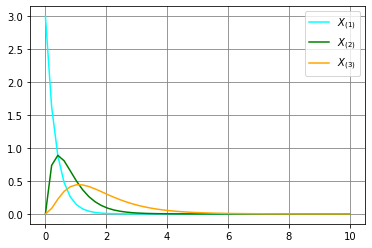
\includegraphics[width=7cm]{plot_1.png}
        \caption{PDF for $X_{(i)}$}
        \label{fig:plot}
    \end{figure}
    
\end{frame}
\begin{frame}{Question}
\begin{block}{gov/stats/2015/statistics-I(1), Q.3(b)}
    Let $Y_1$ denote the first order statistic in a random sample of size $n$ from a distribution that has the pdf, 
    \begin{align}
        f(x) = \nonumber
        \begin{cases}
        e^{-(x-\theta)}&\text{ when } \theta<x<\infty\\
        0 &\text{  otherwise} 
        \end{cases}
    \end{align}
Obtain the distribution of $Z_n = n(Y_1 - \theta)$\\
\end{block}
\end{frame}
\begin{frame}{Solution}
    The problem involves the first order statistic, we begin the solution by finding the cdf of the given distribution:
    \begin{align}
        F(x) &=\displaystyle\int\limits_{-\infty}^{x} f(t) \,dt\\
        &= \displaystyle\int\limits_{-\infty}^{\theta}0\,dt + \displaystyle\int\limits_{\theta}^{x}e^{\theta-t}\,dt\\
        &=\brak{e^{\theta-t}}_{x}^{\theta}\\
        &= 1-e^{\theta-x} \\
        &= 1-f(x) \label{eq_2}
    \end{align}
\end{frame}

\begin{frame}{Solution-CDF}
Let $F_{Z_n}(z)$ and $f_{Z_n}(z)$ be the cdf and pdf for $Z_n$. Calculating the cdf for $Z_n$:
\begin{align}
    F_{Z_n}(z) &= \pr{n(Y_1-\theta)\leq z}\\
    &= \pr{Y_1\leq \frac{z}{n} +\theta}\\
    &= 1-\pr{Y_1\ > \frac{z}{n} +\theta}
\end{align}
Let $\dfrac{z}{n}+\theta=z'$
\begin{align}
    F_{Z_n}&= 1-\pr{X_1>z', X_2>z', ..., X_n>z'}\\
    &= 1-\prod_{i=1}^{n}\pr{X_i>z'}\\
    &= 1-\brak{1-F(z')}^n
\end{align}
\end{frame}

\begin{frame}{Solution-CDF}
    Substituting the expression for $z'$ back,
    \begin{align}
        \implies F_{Z_n}(z) &= 1-\brak{1-F\brak{\frac{z}{n}+\theta}}^n\label{eq_3}\\
    &=1-\brak{f\brak{\frac{z}{n}+\theta}}^n 
    \end{align}
    The expression for the cdf can thus be written as:
\begin{align}
    F_{Z_n}(z) &=
    \begin{cases}
    1-e^{-n\brak{\frac{z}{n}+\theta-\theta}}&\text{when } \theta<\frac{z}{n}+\theta<\infty\\
    0&\text{otherwise}
    \end{cases}\\
    &= \begin{cases}
    1-e^{-z}&\text{when } 0<z<\infty\\
    0 &\text{otherwise}\label{cdf}
    \end{cases}
\end{align}
\end{frame}

\begin{frame}{Solution-PDF}
    Using the cdf in \eqref{cdf} to calculate the pdf:\\
\begin{align}
    f_{Z_n}(z) &= \frac{d}{dz}F_{Z_n}(z)\\
    &=\begin{cases}
    e^{-z}&\text{when } 0<z<\infty\\
    0&\text{otherwise}
    \end{cases}\label{pdf}
\end{align}
\end{frame}
\begin{frame}{Solution-Plots}
The plots for the cdf in \eqref{cdf} and the pdf in \eqref{pdf} are shown below:
 \begin{figure}%
    \centering
    \subfloat[\centering cdf of $Z_n$]{{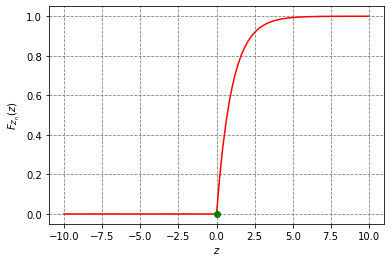
\includegraphics[width=5.5cm]{cdf.png} }}%
    \qquad
    \subfloat[\centering pdf of $Z_n$]{{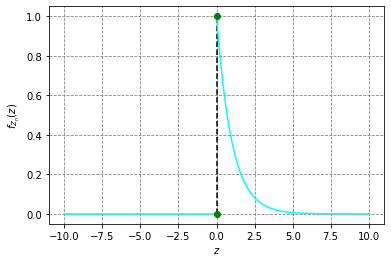
\includegraphics[width=5.5cm]{pdf.png} }}%
    \caption{Plots}%
    \label{fig:example}%
 
\end{figure}
    
\end{frame}






\end{document}

